\chapter{Applikationen und Webseite}
Die Applikationen und die Webseite sollen die Verwendung vom TIMA für möglichst
viele Endnutzer möglich machen.

\section{Webseite}
Die Webseite bzw. das Webfrontend ist die Hauptanlaufstelle für Nutzer. Hierüber kann er sowohl anonym als auch angemeldet Assoziationen eingegeben, Wörter und
deren Assoziationen ansehen und weitere Funktionen wie die Rangliste und andere Statistiken aufrufen.

Das Webfrontend basiert auf Django, wurde zusätzlich zu HTML mit Bootstrap und JQuery erstellt. Zur Visualisierung von Assoziationsgraphen wurde D3.js verwendet.

\section{Applikationen}
Die Applikationen sollen die Verwendung von TIMA ohne Webbrowser ermöglichen. Durch Applikationen wird besonders für mobile Geräte die Nutzung vereinfacht.
In einer erste Variante der Applikation wurden grundlegende Funktionen der
Webseite nachgebaut. Dies diente unter anderem der Entwicklung der API, um etwaige
Fehler im Übertraungsprotokoll aufzuzeigen und zu beheben beziehungsweise Verbesserungsmöglichkeiten zu erhalten.

\subsection{Bibliothek}
Als Bibliothek wurde sich für Qt5 entschieden Aufgrund der weitreichenden
Unterstützung der Bibliothek auf verschiedenen Endgeräten. Hier ist besonders darauf hinzuweisen, das Qt5 sowohl auf Andriod als auch auf iOS läuft und so nicht die gleiche Applikation für beide Betriebssysteme geschrieben werden muss.
Es wurde zudem Java in betracht bezogen, da dies vorrangig auf Mobilen Geräten
Verwendung findet. Allerdings wurde sich aus den eben genannten, sowie Sympathiegründen des Entwicklers
dagegen entschieden.

\subsection{Aufbau}
Die innere Logik wird durch einen Zustandsautomaten dargestellt um
Mehrfachanfragen zu vermeiden und eine einfache Fehlerkorrektur zu ermöglichen.
In \hyperref[fig:uml_automata]{Abbildung \ref*{fig:uml_automata}} wird der Zusammenhang der einzelnen
Zustände angezeigt. Das Wechseln der Zustände wird ausschließlich über die
Signale geregelt, die mit Qt implementiert sind.
\begin{figure}[!h]
	\centering
	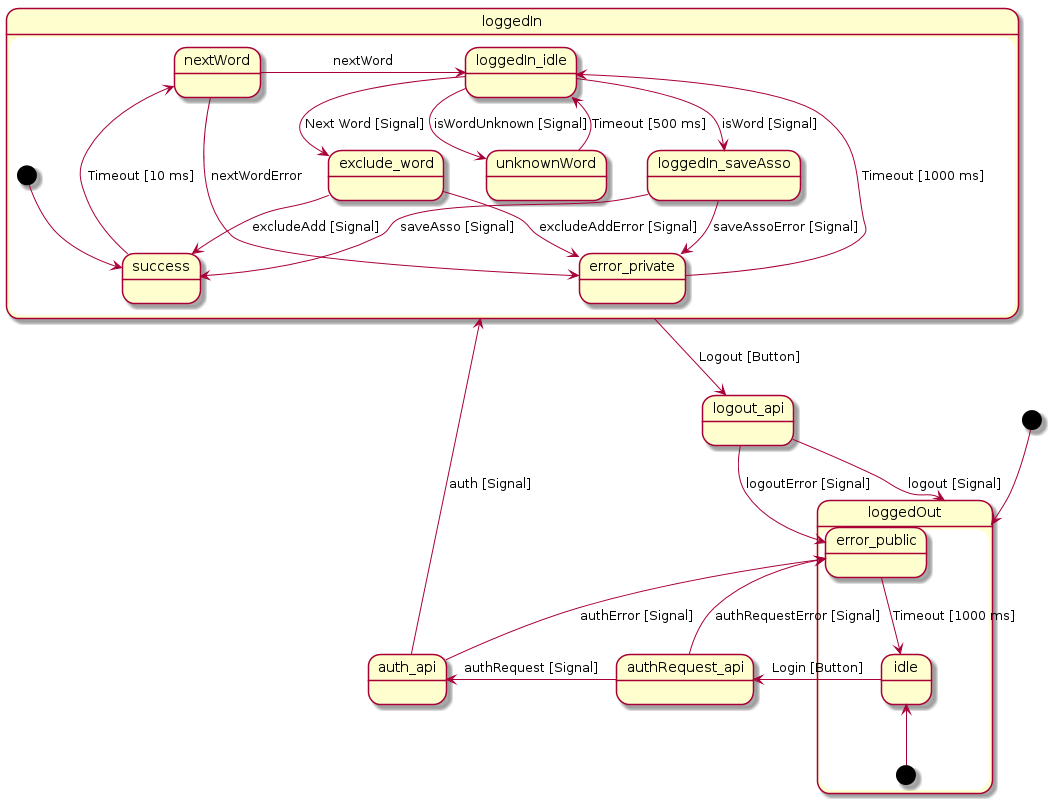
\includegraphics[width=\textwidth]{../UML/app_automata.png}
	\caption{UML State Diagramm des Applikationszustandsautomaten}
	\label{fig:uml_automata}
\end{figure}

\section{Sicherheit}
Die Sicherheit hat bei der Entwicklung eine große Rolle gespielt. Jede Applikation nutzt die in \hyperref[subsec:authentifizierte_anfragen]{Abschnitt \ref*{subsec:authentifizierte_anfragen}} vorgestellte Autorisierungsmethode um mit der API zu kommunizieren.  Dies dient dazu, dass lediglich von TIMA
akzeptierte Applikationen Schreibrechte auf der Datenbank haben. Das Auslesen
der Informationen bleibt davon jedoch unangetastet, sofern es sich nicht um benutzerspezifische Daten handelt, und ist nach wie vor für
jeden offen.
